\documentclass{article}
\usepackage{graphicx} % Required for inserting images
\usepackage{amsmath}
\usepackage{mathalfa}
\usepackage{blindtext}
\usepackage[letterpaper, portrait, margin=0.75in]{geometry}
\usepackage{amssymb}
\usepackage{epsf, subfigure, verbatim, epsfig}
\usepackage{fancyhdr}
\usepackage{calc}
\usepackage{ifthen}
\usepackage{layout}
\usepackage{fancybox}
\usepackage{eurosym}
\usepackage{tabularx}
\usepackage{xspace}
\usepackage{dsfont,mathrsfs}
\usepackage{amssymb}
\usepackage{theorem}
\usepackage{multicol}
\usepackage{float}
\usepackage{tikz}
\usepackage{pgfplots}
\pgfplotsset{compat=1.18}

\title{Homework 3 \\ \large MATH 476}
\author{Ahad Jiva}
\date{April 23, 2025}

\begin{document}

\maketitle
\section*{Exercise 28} 
An investor buys for \$3 a 3-month European call with a strike price of \$30 and sells for \$1 a 3-month
European call with a strike price of \$35. Find the profit from this bull spread in each of the following cases:
\begin{enumerate}
    \item $S_T = \$25$. We know that $K_1 = \$30$ since it is the long position and that $K_2 = \$35$ since it is the short position.
    Then $S_T < K_1 < K_2$. Using the payoff form a bull spread from exercise 27, we know the payoff is 0. Then the profit is $-\$2$.
    \item $S_T = \$34$. Then $K_1 < S_T < K_2$. So we know that the payoff is $S_T - K_1$. So the payoff is \$4. Then the profit is \$2.
    \item $S_T = \$40$. Then $S_T > K_2$. So the payoff is $K_2 - K_1$, or \$5. Then the profit is \$3. 
\end{enumerate}

\section*{Exercise 31}
\begin{flushleft}
Find the payoff from a straddle (long on an ECO and long on an EPO, both same strike price and expiry).
We know the payoff from the long ECO is 
\begin{center}
    $\begin{cases}
        S_T - K & S_T > K \\
        0 & S_T \leq K
    \end{cases}$
\end{center}
and the payoff from the long EPO is
\begin{center}
    $\begin{cases}
        K-S_T & S_T < K \\
        0 & S_T \geq K
    \end{cases}$
\end{center}
Then the total payoff is
\begin{center}
    $\begin{cases}
        S_T - K & S_T > K \\
        K - S_T & S_T \leq K
    \end{cases}$
\end{center}
This can be represented with the following payoff diagram
\begin{center}
    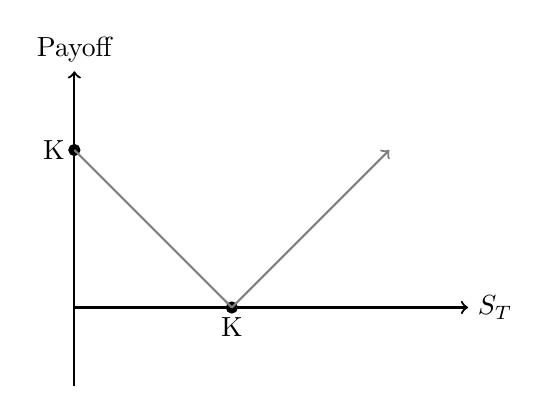
\begin{tikzpicture}
        \draw[black, thick] [->] (-5,1) -- (-5, 5);
        \draw[black, thick] [->] (-5,2) -- (0,2);
        \filldraw[black] (-5,4) circle (2pt) node[anchor=east]{K};
        \filldraw[black] (-3,2) circle (2pt) node[anchor=north]{K};
        \draw[gray, thick] (-5,4) -- (-3,2);
        \draw[gray, thick] [->] (-3,2) -- (-1,4);
        \filldraw[black] (0,2) circle (0pt) node[anchor=west]{$S_T$};
        \filldraw[black] (-5,5) circle (0pt) node[anchor=south]{Payoff};
    \end{tikzpicture}
\end{center}
\end{flushleft}
\break
\section*{Exercise 35}
Initial deposit of \$100, annual interest of 10\%, find value after two years when compounded
\begin{enumerate}
    \item Annually: Then we have $V(2) = (1 + \frac{10}{1})^{2\cdot1} \cdot 100 = \$121$
    \item Monthly: Then we have $V(2) = (1 + \frac{10}{12})^{2\cdot12} \cdot 100 = \$122.03$
\end{enumerate}

\section*{Exercise 36}
Show if $m < k$, then
\begin{center}
    $(1 + \frac{r}{m})^m < (1 + \frac{r}{k})^k$
\end{center}
\begin{flushleft}
    Proof: Let $f(x) = (1 + \frac{r}{x})^x$ for $x > 0$. It is enough to show that $f(x)$ is increasing. Take the natural log of both sides and use log rules to get:
    \begin{center}
        $\ln(f(x)) = \ln((1 + \frac{r}{x})^x) = x\ln(1 + \frac{r}{x})$
    \end{center}
    Now take the derivative of both sides and simplify:
    \begin{center}
        $\frac{1}{f(x)} f'(x) = \ln(1 + \frac{r}{x}) + x(\frac{1}{1+\frac{r}{x}})(-\frac{r}{x^2})$ \\
        $f'(x) = f(x) \big(\ln(1 + \frac{r}{x}) - \frac{r}{x+r}\big)$
    \end{center}
    Observe that $f(x) > 0$, so we just need to show that the other term is positive.
    \begin{center}
        $\ln(1 + \frac{r}{x}) - \frac{r}{x+r} > 0$ \\
        $(x + r) \cdot \ln(1 + \frac{r}{x}) > r$ \\
        $e^{x+r} (1 + \frac{r}{x}) > e^{x+r}$
    \end{center}
    We know this must be true, therefore $f'(x)$ is indeed greater than zero. So $f(x)$ is indeed increasing and we are done. $\square$
\end{flushleft}

\section*{Exercise 37}
Solve $\frac{dV}{dt} = r \cdot V$
\begin{flushleft}
    We can use separation of variables to solve this differential equation.
    \begin{center}
        $\frac{dV}{V} = r \cdot dt$
    \end{center}
    Integrate both sides:
    \begin{center}
        $\int \frac{dV}{V} = \int r \cdot dt$ \\
        $\ln(|v|) = rt + C$ \\
        $V = e^{rt + C} = Ce^{rt}$
    \end{center}
    Now we can use our initial condition to find a specific solution.
    \begin{center}
        $V(0) = 0$ \\
        $V(0) = Ce^0$ \\
        $P = C$
    \end{center}
    Thus $V = Pe^{rt}$.
\end{flushleft}

\section*{Exercise 38}
Continous compounding is given by $V(t)=\lim_{m\rightarrow\infty}\left(1+\frac{r}{m}\right)^{tm}P.$
\begin{enumerate}
    \item Show that $e=\lim_{x\rightarrow\infty}\left(1+\frac{1}{x}\right)^x.$ To start, we can take the natural log of both sides:
        \begin{center}
            $\ln(e) = \ln(\lim_{x\rightarrow\infty}(1 + \frac{1}{x})^x)$ \\
            $1 = \lim_{x\rightarrow\infty}(\ln(1 + \frac{1}{x})^x)$ \\
            $1 = \lim_{x\rightarrow\infty}(x\ln(1 + \frac{1}{x}))$ \\
            $1 = \lim_{x\rightarrow\infty}\left( \frac{\ln(1 + \frac{1}{x})}{\frac{1}{x}}\right)$
        \end{center}
        Now we can use L'Hopital's Rule to evaluate this limit:
        \begin{center}
            $1 = \lim_{x\rightarrow\infty}\left( \frac{\frac{1}{1 + \frac{1}{x}} (\frac{-1}{x^2})}{(\frac{-1}{x^2})} \right)$ \\
            $1 = \lim_{x\rightarrow\infty}(\frac{1}{1 + \frac{1}{x}}) = \frac{1}{1} = 1$
        \end{center}
        Thus we achieve the desired result.
    \item Now we want to obtain a closed form expression for $V(t)$. By using the proof above, we can assert that
        \begin{center}
            $e^r = \lim_{x\rightarrow\infty}(1 + \frac{r}{x})^x$
        \end{center}
        We know that $V(t)=\displaystyle \lim_{m\rightarrow\infty}\left(1+\frac{r}{m}\right)^{tm}P$. We can rewrite this as
        \begin{center}
            $\left( \lim_{m\rightarrow\infty} (1 + \frac{r}{m})^m \right)^t \cdot P = $ \\
            $e^{rt} \cdot P = Pe^{rt}$
        \end{center}
        Thus the closed form for $V(t)$ is $V(t) = Pe^{rt}$, and this matches our result from solving the differential equation.
\end{enumerate}

\end{document}